% ==========================================
% BASE KNOWLEDGES
% ==========================================

\newpage
\chapter{KIẾN THỨC NỀN}

\section{Hệ thống BE-PUM}

\subsection{Kiến trúc của BE-PUM}

\hspace{0.5cm}Hệ thống BE-PUM xây dựng mô hình quá trình thực thi của một tập tin thực thi dựa trên kỹ thuật Dynamic symbolic execution. BE-PUM dựa trên thư viện mã nguồn mở Jackstab để dịch ngược mã nhị phân cho từng câu lệnh hợp ngữ tương ứng với từng câu lệnh thực thi của tập tin và chương trình Z3 để tìm ra đường đi nếu câu lệnh thực thi là một câu lệnh nhảy hoặc nhảy có điều kiện.

\begin{figure}[h]
\centering
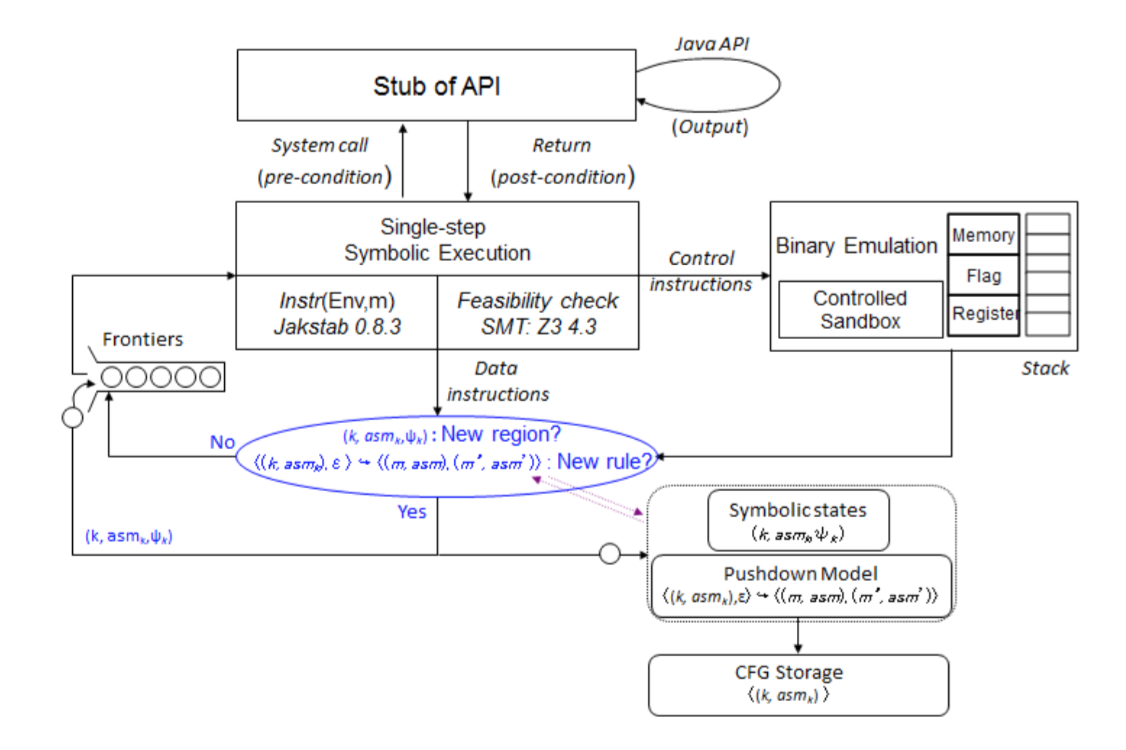
\includegraphics[width=0.7\textwidth]{bepum_architecture}
\caption{Kiến trúc của hệ thống BE-PUM}
\label{fig:BepumArchi}
\end{figure}

\hspace{0.5cm}Kiến trúc của hệ thống BE-PUM bao gồm 3 thành phần chính: symbolic execution, binary emulation và CFG storage. Hình \ref {fig:BepumArchi} mô tả kiến trúc của hệ thống BE-PUM. Trong đó, vai trò của các thành phần này như sau:

\begin{itemize}
\item{Single-step symbolic execution: sử dụng Jackstab để dịch ngược và chuyển đổi thành câu lệnh hợp ngữ tương ứng. Nếu câu lệnh hợp ngữ là câu lệnh chỉ tác động tới môi trường thực thi, cụ thể là các câu lệnh tính toán, câu lệnh ghi hoặc đọc trong bộ nhớ, bao gồm cả stack. Khi đó chỉ có môi trường thực thi được thay đổi và vị trí của câu lệnh tiếp theo chỉ được xác định bằng vị trí của câu lệnh hiện tại và kích thước câu lệnh. Nếu câu lệnh tiếp theo là câu lệnh điều khiển, cụ thể là các câu lệnh gọi hàm, câu lệnh trả về từ hàm, câu lệnh nhảy và câu lệnh nhảy có điều kiện, thì câu lệnh tiếp theo sẽ được tính toán thông qua dynamic symbolic execution.\\}
\item{
\begin{figure}[h]
\centering
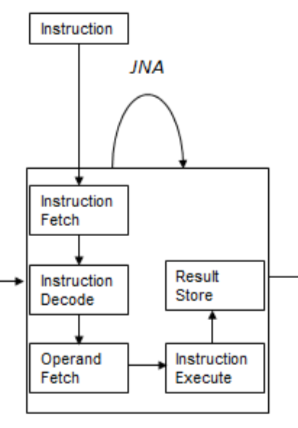
\includegraphics[width=0.3\textwidth]{bepum_binary_emulation}
\caption{Thành phần Binary Emulation trong BE-PUM}
\label{fig:BepumBE}
\end{figure}
Binary emulation: là thành phần quan trọng trong tổng thể kiến trúc của BE-PUM. Để có thể xử lý một câu lệnh hợp ngữ, hệ thống BE-PUM sẽ giả lập các thành phần của hệ thống, cụ thể là mô hình bộ nhớ của BE-PUM, mô hình này bao gồm tập 9 cờ được sử dụng trong hệ thống (AF, CF, DF, IF, OF, PF, SF, TF, và ZF), tập 20 thanh ghi (EAX, EBX, ECX, EDX, ESI, EDI, ESP, EBP, CS, DS, ES, FS, GS, SS, EIP, EFLAGS và 8 thanh ghi debug DRO, DR1, DR2, DR3, DR4, DR5, DR6, DR7, DR8), tập các giá trị bộ nhớ được lưu trữ trong đó một phần của bộ nhớ cho stack được giới hạn bởi thanh ghi esp và thanh ghi ebp. Bộ nhớ được giả lập trong BE-PUM được lưu trữ dưới dạng từng byte một. Ngoài việc giả lập câu lệnh hợp ngữ, thì API cũng được giả lập thông qua sử dụng Java Native Access cho phép gọi trực tiếp từ các thư viện liên kết động, trong đó giá trị trả về của các API sẽ được lưu trữ trong các thanh ghi tương ứng. Đối với các API đặc biệt tác động trực tiếp đến môi trường thực, một sandbox sẽ được xây dựng cho quá trình xử lý các API này. Ngoài ra, các API được sử dụng như một phần của kỹ thuật anti-reversing, anti-debugging, giá trị trả về sẽ là một giá trị symbolic. Hình \ref {fig:BepumBE} mô tả các quá trình xử lý một câu lệnh thực thi trong hệ thống BE-PUM.\\
}
\item{CFG storage: được sử dụng để lưu trữ một CFG node và CFG edge sau khi được tính toán chính xác. CFG storage sẽ được sử dụng để xây dựng mô hình quá trình thực thi cuối cùng của tập tin được phân tích.}
\end{itemize}

\subsection{Mô hình của BE-PUM}
\hspace{0.5cm}Kết quả của quá trình phân tích một tập tin thực thi là một mô hình quá trình thực thi, mô hình được sinh ra bởi hệ thống BE-PUM được biểu diễn dưới dạng Control Flow Graph hay CFG của chương trình.\\

\hspace{0.5cm}Một CFG là một tập của các node và edge. Trong đó một node của CFG bao gồm địa chỉ của câu lệnh và câu lệnh hợp ngữ tại địa chỉ đó, một edge của CFG là cạnh nối giữa 2 node của CFG.

\begin{code}
\begin{lstlisting}[captionpos=b,caption={Ví dụ về một đoạn mã thực thi},label={lst:SampleExe},frame=single]
00401000	pushl 0x00401007
00401005	jne 0x0040101A
0040100A 	movl fs:[0],esp			
\end{lstlisting}
\end{code}

\hspace{0.5cm}Với đoạn mã \ref {lst:SampleExe}, quá trình phân tích trên hệ thống BE-PUM sẽ sinh ra được mô hình của đoạn mã thực thi hay CFG của chương trình thực thi trên như sau:

\begin{figure}
\centering
\begin{tikzpicture}[shorten >=1pt,node distance=2cm,on grid,auto] 
   	\node[cfgstate,align=center](s_1){0x00401000\\\ pushl 0x00401007}; 
   	\node[cfgstate,align=center](s_2)[below of=s_1]{0x00401005\\\ jne 0x0040101A};
   	\node[cfgstate,align=center](s_3)[below of=s_2]{0x0040100A\\\ movl \%fs:[0],\%esp};
    \path[-{>[scale=2,length=3,width=3]}] 
    (s_1) edge node {} (s_2)
  	(s_2.east) edge [bend right=60] node {} (s_1.east)
    (s_2) edge node {} (s_3);	  
\end{tikzpicture}
\label{fig:SampleCFG}
\caption{CFG được sinh ra từ đoạn mã thực thi \ref {lst:SampleExe}}
\end{figure}

\subsection{Hạn chế của BE-PUM}

\hspace{0.5cm}Một số những hạn chế của hệ thống BE-PUM bao gồm:

\begin{itemize}
\item{Số lượng các câu lệnh hợp ngữ là rất lớn khoảng hơn 1000 câu lệnh và số lượng API là 4000. Tuy nhiên hiện tại BE-PUM chỉ hõ trợ được 200 câu lệnh và 400 API. Do đó đối với các malware hay packer sử dụng những câu lệnh hay API không được hỗ trợ, BE-PUM sẽ không thể phân tích tiếp tục được và do đó quá trình phân tích sẽ kết thúc.\\}
\item{Đối với những malware hay packer sử dụng những vòng lặp lớn hơn 1 tỷ lần thì quá trình phân tích trên BE-PUM sẽ kết thúc. Do đó khi gặp một vòng lặp với số lượng lớn thì quá trình phân tích sẽ tiếp tục được phân tích trên một đường thực thi khác.\\}
\item{Trong thực tế, trước khi thực thi tại entry point của chương trình, một số xử lý từ hệ điều hành sẽ được thực hiện qua đó tác động đến các giá trị thanh ghi, bộ nhớ và stack tại entry point. Do đó, khi quá trình phân tích bắt đầu, tại vị trí entry point, hệ thống BE-PUM sẽ mặc định thiết lập các giá trị mặc định cho stack bao gồm: địa chỉ chứa mã ASCII của tên tập tin, địa chỉ hàm xử lý exception của hệ thống, và giá trị trả về là một giá trị bất kì thuộc địa chỉ kernel.\\}
\item{Ngoài ra, các giá trị cờ cũng được thiết lập cụ thể như mô tả trong bảng \ref {table:BepumInitFlag}. Đối với các thanh ghi EAX, CS, DS, ES, FS, GS, SS, EFLAGS được thiết lập giá trị symbolic, các thanh ghi được thiết lập như mô tả trong bảng \ref {table:BepumInitReg}.
}
\end{itemize}

\begin{longtable}{ | m{2cm} | m{5cm} | }
\hline 
CF & False\\
\hline 
PF & True\\
\hline 
AF & False\\
\hline 
ZF & True\\
\hline 
SF & False\\
\hline 
TF & False\\
\hline 
DF & False\\
\hline 
OF & False\\
\hline 
IF & False\\
\hline
\caption{Các giá trị cờ được khởi tạo mặc định trong hệ thống BE-PUM}
\label{table:BepumInitFlag}
\end{longtable}

\begin{longtable}{ | m{5cm} | m{5cm} | }
\hline 
EIP, EDX & Địa chỉ entry point\\
\hline
ESP & Địa chỉ đỉnh của stack\\
\hline
EBP & Địa chỉ cơ sở của stack\\
\hline
ECX, EDI, ESI & 0\\
\hline
EBX & Địa chỉ PEB\\
\hline
\caption{Các giá trị thanh ghi được khởi tạo mặc định trong hệ thống BE-PUM}
\label{table:BepumInitReg}
\end{longtable}

\section{Model Checking và NuSMV}

\subsection{Model Checking}

\subsection{CTL và LTL}

\subsection{Kiểm tra mô hình với NuSMV}

\section{Các kỹ thuật chính của Packer}

